\chapter{小波变换}
\label{chap:wavelet-transform}

第~\ref{chap:functions-as-vectors}章把函数看成一条无限长的向量$[\ldots,f(x),\ldots]$，它的每个分量只报告一个点上的取值。第~\ref{chap:fourier-transform}章换到三角函数基，每个坐标报告一个频率的强度，却要用整个周期上的积分才能读出。这两种坐标各走一个极端：前者只知道位置，后者只知道频率。

一段记录大部分时间平稳，只在少数位置突然跳变，这样的函数放在频率坐标里并不省事，因为一处跳变会让所有频率的系数都不为零。我们希望有一组基，它的坐标同时带着尺度和位置两个标号：先记录整体水平，再逐层记录“这一块的左半和右半相差多少”。这样，平稳区域的细节接近零，一处跳变在每一层只影响覆盖它的少数几块。

小波系数就是这样的坐标：函数这条无限维向量，换到一组多尺度标准正交基之后读出的分量。本章的问题是这组基怎样造出来，它在什么意义下能重构原函数，以及定义域有边界时要做什么调整。

全章从能手算的情形开始。第~\ref{sec:wavelet-finite-haar}节对$2^J$个取值反复求平均与半差，把这个过程整理成$\mathbb R^{2^J}$中的一次正交换基。第~\ref{sec:wavelet-scaling-detail}节把这些取值放回区间$[0,1]$上的分段常数函数，说明每一步换了哪组基函数。第~\ref{sec:wavelet-interval-expansion}节让层数趋于无穷，证明这组基在$L^2([0,1])$中完备。

后三节把构造推广出去。第~\ref{sec:wavelet-real-line}节在全实轴上建立一般的正交多分辨率结构，并讨论比Haar更光滑、能抵消更多多项式的小波。第~\ref{sec:wavelet-boundary}节处理基函数跨过区间端点的问题。第~\ref{sec:wavelet-fourier-comparison}节在同一个周期区间上比较Fourier坐标和小波坐标。

本章使用第~\ref{chap:function-inner-product-spaces}章的正交投影与正交展开，以及第~\ref{chap:fourier-transform}章的Fourier级数。截断误差随项数怎样变化的定量结论在第~\ref{chap:function-approximation}章研究，用小波系数刻画函数正则性的Besov范数在第~\ref{chap:besov-spaces}章建立。

\section{有限Haar变换}
\label{sec:wavelet-finite-haar}

取非负整数$J$，把区间$[0,1)$等分成$N=2^J$段，每段记录一个数，得到向量$\bm a=(a_0,\ldots,a_{N-1})$。这是第~\ref{chap:functions-as-vectors}章函数向量最简单的情形：输入只有$N$个，函数就是$\mathbb R^N$中的一个点。

我们想把这$N$个数改写成两类信息：整体有多高，以及各处在不同尺度上怎样起伏；并且改写以后还能原样拼回去。本节全部在$\mathbb R^N$中计算。

\subsection{逐层平均与差值}
\label{sec:wavelet-average-difference}

\paragraph{一对数的平均与半差}
从两个数开始。相邻取值$a,b$可以换成它们的平均与半差：
\begin{equation}
 s=\frac{a+b}{2},\qquad d=\frac{a-b}{2}.
 \label{eq:wavelet-average-difference}
\end{equation}
$s$记录这两个数共同的水平，$d$记录它们相对平均各偏离多少。

反过来，把两式相加、相减，就得到
\[
 a=s+d,\qquad b=s-d.
\]
所以这一步没有丢失信息，只是换了记法。若$a=b$，则$d=0$：没有起伏的地方，差值就是零。

\paragraph{逐层分解}
对长度$N=2^J$的向量，先把分量两两分组，得到$N/2$个平均和$N/2$个半差。半差保存下来，平均组成一个长度减半的新向量，再对它重复同一步。做完$J$步后只剩一个数，即全部取值的平均。

保存下来的半差个数是
\[
 \frac N2+\frac N4+\cdots+1=N-1,
\]
连同总平均恰好$N$个数，与原向量的分量一样多。恢复时按相反次序进行：从总平均和最粗一层的半差算出两个平均，再与下一层的半差配合得到四个平均，直到恢复全部$N$个取值。每一步都只用加减，所以整个分解是可逆的线性变换。

\begin{example}[四个取值的平均与半差]
\label{ex:wavelet-four-values-average}
取$\bm a=(2,4,8,6)$。第一步把相邻两对分别换成平均和半差：
\[
 (2,4)\mapsto(3,-1),\qquad(8,6)\mapsto(7,1).
\]
第二步对两个平均$(3,7)$再做一次：
\[
 (3,7)\mapsto(5,-2).
\]
于是原向量被记为总平均$5$、两半之间的半差$-2$，以及细层半差$-1,1$。

恢复时先由总平均和粗层半差得到两半的平均：
\[
 5+(-2)=3,\qquad 5-(-2)=7.
\]
再由细层半差得到原来的四个取值：
\[
 3+(-1)=2,\quad3-(-1)=4,\quad7+1=8,\quad7-1=6.
\]
\end{example}

图~\ref{fig:wavelet-average-tree}把这个例子画成了一棵树。沿树向下，每一层的绿框只把平均继续往下传，黄框则留在原地不再变动，这就是逐层分解“只继续处理平均”的含义。

\begin{BookInlineFigure}
  \centering
  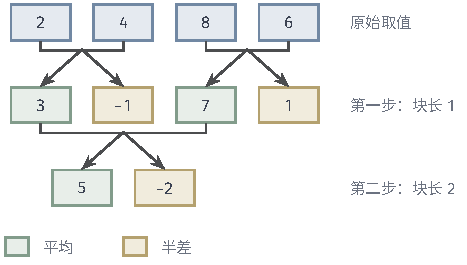
\includegraphics[width=79.07mm]{figures/04-spaces-measures-and-geometry/03-function-spaces/tikz/wavelet-average-tree/figure.pdf}
  \caption{对$(2,4,8,6)$的逐层平均与半差。蓝框是原始取值，绿框是平均，黄框是半差。每一步把一对框换成一个平均和一个半差，半差不再变动，平均进入下一步。}
  \label{fig:wavelet-average-tree}
\end{BookInlineFigure}

\paragraph{差值记录的尺度与位置}
每个半差都对应一个“块”和这一块的左右两半。细层的$-1$只比较$a_0$与$a_1$，块长为一段；粗层的$-2$比较前两段的平均$3$与后两段的平均$7$，块长为两段。块的长短给出尺度，块的位置给出位置，块越短，半差描述的变化越局部。

局部性可以直接检验。把$a_2$从$8$改成$9$，得到$(2,4,9,6)$。第一步的半差和平均变成
\[
 (2,4)\mapsto(3,-1),\qquad(9,6)\mapsto\Bigl(\frac{15}2,\frac32\Bigr).
\]
第二步对平均$(3,15/2)$再做一次，得到
\[
 \Bigl(3,\frac{15}2\Bigr)\mapsto\Bigl(\frac{21}4,-\frac94\Bigr).
\]
比较前后两组数，比较$a_0$与$a_1$的半差$-1$不变，变化的只有包含第$2$段的那些块：细层的$1$变成$3/2$，粗层的$-2$变成$-9/4$，总平均$5$变成$21/4$。一处取值的改动在每一层只影响一个系数。

\subsection{正交变换与逆变换}
\label{sec:wavelet-orthogonal-transform}

上一小节的新坐标已经能够恢复原向量，但还不是一组标准正交基下的坐标，因为它没有保持平方和。由式~\eqref{eq:wavelet-average-difference}直接计算，
\[
 s^2+d^2=\frac{(a+b)^2+(a-b)^2}{4}=\frac{a^2+b^2}{2}.
\]
每做一步，平方和减半。第~\ref{chap:function-inner-product-spaces}章的正交展开要求坐标平方和等于长度的平方，所以我们把两个新系数都乘以$\sqrt2$。

\paragraph{二阶正交变换}
把一对取值$(a,b)$换成
\begin{equation}
 \begin{bmatrix}s\\d\end{bmatrix}
 =\bm H_2\begin{bmatrix}a\\b\end{bmatrix},\qquad
 \bm H_2=\frac{1}{\sqrt2}\begin{bmatrix}1&1\\1&-1\end{bmatrix}.
 \label{eq:wavelet-h2}
\end{equation}
即$s=(a+b)/\sqrt2$，$d=(a-b)/\sqrt2$。这里沿用记号$s,d$，它们比式~\eqref{eq:wavelet-average-difference}中的量都大$\sqrt2$倍。

直接相乘可以核对
\[
 \bm H_2^{\top}\bm H_2=\frac12\begin{bmatrix}2&0\\0&2\end{bmatrix}=\bm I.
\]
所以$\bm H_2$是正交矩阵，这一步保持平方和，逆矩阵等于转置。$\bm H_2$还是对称的，于是逆变换与正变换形式相同。正交矩阵的这些性质见\BookChapterRef{chap:inner-product-spaces}{卷二第4章“内积空间”}。

\paragraph{多层变换}
对长度$N=2^J$的向量，第一层对全部$N/2$对取值作用$\bm H_2$，得到$N/2$个粗系数和$N/2$个细节系数。第二层只对粗系数两两作用$\bm H_2$，细节系数原样保留；依此类推，共做$J$层。

每一层在被处理的坐标上是若干个$\bm H_2$拼成的分块对角正交矩阵，在其余坐标上是恒等，所以每一层都是正交变换，它们的复合也是正交变换。我们把输出排成“最粗项在前，细节由粗到细”：先写最后剩下的一个粗系数，再写最粗一层的细节，最后写第一层得到的$N/2$个细节。

记这样得到的矩阵为$\bm W_N$，称$\bm c=\bm W_N\bm a$为$\bm a$的\term{Haar变换}（Haar transform）。由正交性，
\begin{equation}
 \lVert\bm c\rVert_2=\lVert\bm a\rVert_2,\qquad \bm a=\bm W_N^{\top}\bm c.
 \label{eq:wavelet-finite-haar-isometry}
\end{equation}
计算量也很小：第一层处理$N/2$对，第二层$N/4$对，总共$N-1$对。每对只做两次加减和两次乘以$1/\sqrt2$，所以运算次数与$N$成正比。

\begin{example}[四个取值的正交Haar变换]
\label{ex:wavelet-four-values-orthogonal}
仍取$\bm a=(2,4,8,6)$。第一层把两对取值分别作用$\bm H_2$：
\[
 (2,4)\mapsto(3\sqrt2,-\sqrt2),\qquad(8,6)\mapsto(7\sqrt2,\sqrt2).
\]
第二层把粗系数$(3\sqrt2,7\sqrt2)$再作用一次：
\[
 (3\sqrt2,7\sqrt2)\mapsto\Bigl(\frac{10\sqrt2}{\sqrt2},\frac{-4\sqrt2}{\sqrt2}\Bigr)=(10,-4).
\]
按约定排序，得到
\[
 \bm c=(10,-4,-\sqrt2,\sqrt2).
\]

这四个数也可以一次写成矩阵乘法：
\[
 \bm W_4=\begin{bmatrix}
 1/2&1/2&1/2&1/2\\
 1/2&1/2&-1/2&-1/2\\
 1/\sqrt2&-1/\sqrt2&0&0\\
 0&0&1/\sqrt2&-1/\sqrt2
 \end{bmatrix}.
\]
各行长度为$1$且两两正交。平方和核对如下：
\[
 4+16+64+36=120,\qquad 100+16+2+2=120.
\]

逆变换$\bm W_4^{\top}\bm c$逐分量计算，四个分量依次是
\[
 5-2-1=2,\quad5-2+1=4,\quad5+2+1=8,\quad5+2-1=6.
\]
这恢复了原向量。
\end{example}

\paragraph{矩阵的各行就是新基}
$\bm c=\bm W_4\bm a$的第$i$个分量是$\bm W_4$第$i$行与$\bm a$的点积。所以$\bm W_4$的四行组成$\mathbb R^4$的一组新标准正交基，而$\bm c$是$\bm a$在这组基下的坐标。

第一行是常数向量，读取整体水平；第二行把前后两半相减，读取最粗的起伏；后两行只在相邻两个位置非零，读取最细的局部起伏。从标准基换到这组基，向量本身没有变，变的只是读取它的方式。

\paragraph{与平均和半差的关系}
比较两个例子，对应系数之间的比例是
\[
 10=2\times5,\quad-4=2\times(-2),\quad-\sqrt2=\sqrt2\times(-1),\quad\sqrt2=\sqrt2\times1.
\]
一般地，若一个系数对应由$2^m$个原始取值组成的块，则正交变换给出的系数等于$2^{m/2}$乘以该块的平均或半差。

对$m$归纳可以验证这一点。两个长为$2^{m-1}$的子块，平均记为$s_L,s_R$，归纳假设说它们的粗系数是$2^{(m-1)/2}s_L$和$2^{(m-1)/2}s_R$。再作用$\bm H_2$，第一个分量是
\[
 \frac{2^{(m-1)/2}(s_L+s_R)}{\sqrt2}=2^{m/2}\cdot\frac{s_L+s_R}{2},
\]
这正是$2^{m/2}$乘以大块的平均，半差同理。两种算法携带相同的信息，区别只在每个系数的比例因子，正交版本用这些因子换来了长度不变。

\section{尺度空间与细节空间}
\label{sec:wavelet-scaling-detail}

上一节的$2^J$个取值可以看成一个函数：在区间$[0,1)$的第$k$段上取常值$a_k$。这样，平均与差值就变成了对函数的运算，Haar变换就变成了在同一个函数空间中更换基函数。本节先建立由分段常数函数组成的尺度空间，再用正交补定义细节空间，最后核对取值向量与函数坐标之间相差的归一化因子。全节在$L^2([0,1])$中讨论，内积为$\langle f,g\rangle=\int_0^1\overline{f(x)}g(x)\,dx$，按第~\ref{chap:inner-product-spaces}章的约定对第一个变量共轭线性；本章出现的基函数都是实值的。

\subsection{尺度空间}
\label{sec:wavelet-scaling-spaces}

对整数$j\geq0$和$0\leq k<2^j$，记
\[
I_{j,k}=\bigl[k2^{-j},(k+1)2^{-j}\bigr),
\]
称为第$j$层的\term{二进区间}（dyadic interval）。第$j$层的$2^j$个二进区间互不相交，并起来是$[0,1)$。尺度$j$决定区间长度$2^{-j}$，位置$k$决定区间落在哪里。端点$x=1$只是一个零测集，在$L^2([0,1])$中不影响任何元素，所以下面不再区分$[0,1)$与$[0,1]$。

\begin{definition}[Haar尺度空间]
\label{def:wavelet-scaling-space}
对整数$j\geq0$，令$V_j$为$L^2([0,1])$中在每个$I_{j,k}$上几乎处处取常值的元素组成的子空间，称为第$j$层的\term{尺度空间}（scaling space）。令
\[
\varphi_{j,k}=2^{j/2}\mathbf{1}_{I_{j,k}}\qquad(0\leq k<2^j).
\]
\end{definition}

因子$2^{j/2}$的作用是归一化。不同的$\varphi_{j,k}$支撑在不相交的区间上，内积为零；而$\lVert\varphi_{j,k}\rVert_2^2=2^j\cdot2^{-j}=1$。$V_j$中的每个元素都是$\sum_kb_k\mathbf{1}_{I_{j,k}}$的形式，所以$\{\varphi_{j,k}\}_{0\leq k<2^j}$是$V_j$的标准正交基，$\dim V_j=2^j$。有限维子空间是闭的，第~\ref{chap:inner-product-spaces}章的正交投影可以直接使用。

\paragraph{嵌套}
每个第$j$层区间恰好是两个第$j+1$层区间的并：$I_{j,k}=I_{j+1,2k}\cup I_{j+1,2k+1}$。在$I_{j,k}$上取常值的函数，在这两个子区间上当然也取常值，所以
\[
V_0\subset V_1\subset V_2\subset\cdots .
\]
层级越高，允许的分段越细，空间越大。$V_0$只含常数函数。

\paragraph{投影就是取区间平均}
$L^2([0,1])$中的函数在有限测度区间上可积（由Cauchy--Schwarz不等式，$\int_I|f|\leq\lvert I\rvert^{1/2}\lVert f\rVert_2$），所以每个区间上的平均有意义。设$P_j$是到$V_j$的正交投影。用标准正交基写出，
\begin{equation}
P_jf=\sum_{k=0}^{2^j-1}\langle\varphi_{j,k},f\rangle\varphi_{j,k}
=\sum_{k=0}^{2^j-1}\Bigl(2^j\int_{I_{j,k}}f(x)\,dx\Bigr)\mathbf{1}_{I_{j,k}} .
\label{eq:wavelet-projection-average}
\end{equation}
括号中的数正是$f$在$I_{j,k}$上的平均。所以$P_jf$在每个第$j$层区间上取$f$在该区间的平均值，它是$V_j$中离$f$最近的函数。例如$f(x)=x$时，$P_0f\equiv1/2$，$P_1f$在$[0,1/2)$上为$1/4$、在$[1/2,1)$上为$3/4$。

\subsection{细节空间}
\label{sec:wavelet-detail-spaces}

从$V_j$到$V_{j+1}$，空间多出了$2^{j+1}-2^j=2^j$维。多出来的部分应当恰好记录“每个第$j$层区间的左右两半有何不同”，因为在第$j$层这一差别被平均掉了。用正交补把这部分单独取出。

\begin{definition}[Haar细节空间与Haar函数]
\label{def:wavelet-detail-space}
对整数$j\geq0$，令$W_j=V_{j+1}\cap V_j^{\perp}$，称为第$j$层的\term{细节空间}（detail space）。令
\[
\psi=\mathbf{1}_{[0,1/2)}-\mathbf{1}_{[1/2,1)},\qquad
\psi_{j,k}=2^{j/2}\bigl(\mathbf{1}_{I_{j+1,2k}}-\mathbf{1}_{I_{j+1,2k+1}}\bigr)\qquad(0\leq k<2^j),
\]
称$\psi_{j,k}$为\term{Haar函数}（Haar function）。
\end{definition}

$\psi_{j,k}$在$I_{j,k}$的左半取$2^{j/2}$、右半取$-2^{j/2}$，在其余位置为零。用变量代换可以写成$\psi_{j,k}(x)=2^{j/2}\psi(2^jx-k)$，所以全部Haar函数都由同一个$\psi$平移、缩放而来。

\begin{theorem}[细节空间的标准正交基]
\label{thm:wavelet-detail-basis}
对每个$j\geq0$，$\{\psi_{j,k}\}_{0\leq k<2^j}$是$W_j$的标准正交基，并且$V_{j+1}=V_j\oplus W_j$，两者正交。
\end{theorem}

\begin{proof}
$\psi_{j,k}$在每个第$j+1$层区间上取常值，属于$V_{j+1}$。它与$\varphi_{j,k'}$正交：$k'\neq k$时支撑不交；$k'=k$时
\[
\langle\varphi_{j,k},\psi_{j,k}\rangle=2^{j}\bigl(2^{-j-1}-2^{-j-1}\bigr)=0 .
\]
所以$\psi_{j,k}\in V_j^{\perp}$，从而$\psi_{j,k}\in W_j$。不同的$\psi_{j,k}$支撑不交，且$\lVert\psi_{j,k}\rVert_2^2=2^j\cdot2^{-j}=1$，它们是标准正交的。

有限维空间$V_{j+1}$中，闭子空间$V_j$的正交补$W_j$满足$V_{j+1}=V_j\oplus W_j$，维数为$2^{j+1}-2^j=2^j$。$W_j$中有$2^j$个标准正交向量，它们线性无关，因而构成$W_j$的基。
\end{proof}

也可以直接看出$V_{j+1}$中的每个函数都能用两组基表示：由定义，
\[
\mathbf{1}_{I_{j+1,2k}}=\frac{2^{-j/2}}{2}\bigl(\varphi_{j,k}+\psi_{j,k}\bigr),\qquad
\mathbf{1}_{I_{j+1,2k+1}}=\frac{2^{-j/2}}{2}\bigl(\varphi_{j,k}-\psi_{j,k}\bigr).
\]
这两个式子正是平均与半差的函数版本：一个细区间上的指示函数，等于所在粗区间的平均部分加上或减去一个细节。

\paragraph{逐层分解}
把定理~\ref{thm:wavelet-detail-basis}反复用于$V_J,V_{J-1},\ldots,V_1$，得到正交直和分解
\begin{equation}
V_J=V_0\oplus W_0\oplus W_1\oplus\cdots\oplus W_{J-1}.
\label{eq:wavelet-finite-decomposition}
\end{equation}
维数核对为$1+1+2+\cdots+2^{J-1}=2^J$。相应地，$\{\varphi_{0,0}\}\cup\{\psi_{j,k}:0\leq j<J,\ 0\leq k<2^j\}$是$V_J$的另一组标准正交基。

用投影写出，到$W_j$的正交投影是$P_{j+1}-P_j$。所以第$j$层细节就是“用第$j+1$层区间平均表示”与“用第$j$层区间平均表示”之差，正是较粗表示中缺少的局部差异。仍以$f(x)=x$为例，$P_1f-P_0f$在左半为$-1/4$、右半为$1/4$。另一方面$\langle\psi_{0,0},f\rangle=\int_0^{1/2}x\,dx-\int_{1/2}^1x\,dx=1/8-3/8=-1/4$，于是$\langle\psi_{0,0},f\rangle\psi_{0,0}$在两半上分别为$-1/4$和$1/4$，两种算法一致。

\subsection{值向量与函数坐标}
\label{sec:wavelet-values-coordinates}

现在把第~\ref{sec:wavelet-finite-haar}节的有限计算准确地放进$V_J$。设$f=\sum_{k=0}^{N-1}a_k\mathbf{1}_{I_{J,k}}$，$N=2^J$，即$f$在第$k$段上取值$a_k$。它的平方积分是
\[
\lVert f\rVert_2^2=\sum_{k=0}^{N-1}a_k^2\cdot2^{-J},
\]
与取值向量的欧氏平方和差一个因子$2^{-J}$。原因是每段的长度为$2^{-J}$。改用标准正交基表示，$f=\sum_k(2^{-J/2}a_k)\varphi_{J,k}$，所以$f$在基$\{\varphi_{J,k}\}$下的坐标是$2^{-J/2}\bm a$。这个坐标向量的欧氏长度才等于$\lVert f\rVert_2$。

\paragraph{一步变换就是一次换基}
在相邻两个细区间上，由定义有
\[
\varphi_{j,k}=\frac{\varphi_{j+1,2k}+\varphi_{j+1,2k+1}}{\sqrt2},\qquad
\psi_{j,k}=\frac{\varphi_{j+1,2k}-\varphi_{j+1,2k+1}}{\sqrt2}.
\]
若$f$在这两个细区间上的部分是$c_0\varphi_{j+1,2k}+c_1\varphi_{j+1,2k+1}$，代入上式验证可得
\[
c_0\varphi_{j+1,2k}+c_1\varphi_{j+1,2k+1}
=\frac{c_0+c_1}{\sqrt2}\varphi_{j,k}+\frac{c_0-c_1}{\sqrt2}\psi_{j,k}.
\]
右端的两个系数正是式~\eqref{eq:wavelet-h2}中$\bm H_2$作用在$(c_0,c_1)$上的结果。所以对坐标向量$2^{-J/2}\bm a$作有限Haar变换，得到的正是$f$在基$\{\varphi_{0,0}\}\cup\{\psi_{j,k}\}$下的坐标，排序与第~\ref{sec:wavelet-orthogonal-transform}小节的约定一致：先是$\langle\varphi_{0,0},f\rangle$，再是由粗到细的$\langle\psi_{j,k},f\rangle$。

\begin{example}[四段函数的Haar系数]
\label{ex:wavelet-four-values-function}
取$J=2$，$f$在四段上依次取$2,4,8,6$。坐标向量是$2^{-1}\bm a=(1,2,4,3)$。第一层得$(3/\sqrt2,-1/\sqrt2)$与$(7/\sqrt2,1/\sqrt2)$，第二层把$(3/\sqrt2,7/\sqrt2)$换成$(5,-2)$，所以
\[
\bigl(\langle\varphi_{0,0},f\rangle,\langle\psi_{0,0},f\rangle,\langle\psi_{1,0},f\rangle,\langle\psi_{1,1},f\rangle\bigr)=\Bigl(5,-2,-\frac{1}{\sqrt2},\frac{1}{\sqrt2}\Bigr).
\]
这些数也可以直接积分核对。$\langle\varphi_{0,0},f\rangle=\int_0^1f=(2+4+8+6)/4=5$是$f$的平均；$\langle\psi_{0,0},f\rangle=(2+4)/4-(8+6)/4=-2$；$\langle\psi_{1,0},f\rangle=\sqrt2(2/4-4/4)=-1/\sqrt2$；$\langle\psi_{1,1},f\rangle=\sqrt2(8/4-6/4)=1/\sqrt2$。

它们与例~\ref{ex:wavelet-four-values-orthogonal}的欧氏系数$(10,-4,-\sqrt2,\sqrt2)$逐项相差因子$2^{-J/2}=1/2$。能量核对为$\lVert f\rVert_2^2=(4+16+64+36)/4=30$与$25+4+1/2+1/2=30$。此时保持的是函数的平方积分，而不是取值向量的平方和。
\end{example}

这个归一化在实际计算中容易混淆：直接对取值向量作正交Haar变换，得到的数要再乘以$2^{-J/2}$才是$L^2$中的系数。若只关心系数的相对大小，因子无关紧要；若要用系数估计函数的$L^2$误差，就必须带上它。

\section{区间上的Haar展开}
\label{sec:wavelet-interval-expansion}

有限层级的空间$V_J$只含在第$J$层二进区间上取常值的函数。$f(x)=x$这样简单的函数也不在任何$V_J$中，因为它在每个区间内都在变化。要用Haar函数表示一般的$L^2([0,1])$函数，必须让层级无限增加，并说明这样做确实能逼近任意元素。本节先证明尺度空间的并是稠密的，再用第~\ref{chap:inner-product-spaces}章的正交展开得到系数、重构与能量等式。

\subsection{尺度空间的稠密性}
\label{sec:wavelet-scaling-density}

我们要证明：任给$f\in L^2([0,1])$和$\varepsilon>0$，存在某个$j$和$g\in V_j$，使$\lVert f-g\rVert_2<\varepsilon$。$V_j$中的元素称为二进阶梯函数。思路是把一般函数逐步化简：先截去大值，再换成简单函数，再换成有限个区间的指示函数，最后把区间端点移到二进点上。每一步的误差都可以任意小。

\begin{theorem}[二进阶梯函数的稠密性]
\label{thm:wavelet-dyadic-dense}
$\bigcup_{j\geq0}V_j$在$L^2([0,1])$中稠密。因此对每个$f\in L^2([0,1])$，
\[
\lVert f-P_jf\rVert_2\to0\qquad(j\to\infty),
\]
并且$\lVert f-P_jf\rVert_2$随$j$单调不增。
\end{theorem}

\begin{proof}
\emph{第一步：截去大值。}对$M>0$，令$f_M=f\mathbf{1}_{\{\lvert f\rvert\leq M\}}$。逐点有$f_M\to f$（$M\to\infty$），且$\lvert f-f_M\rvert^2\leq\lvert f\rvert^2$可积。由控制收敛定理，$\lVert f-f_M\rVert_2\to0$。所以只需逼近有界可测函数。

\emph{第二步：换成简单函数。}由第~\ref{chap:measure}章的简单函数逼近，有界可测函数$f_M$（复值时分别处理实部与虚部）可以被只取有限个值的简单函数一致逼近。区间$[0,1]$的测度为$1$，一致误差不超过$\delta$时，$L^2$误差也不超过$\delta$。所以只需逼近简单函数，又由线性只需逼近单个指示函数$\mathbf{1}_E$，$E\subset[0,1]$可测。

\emph{第三步：换成有限个区间。}由第~\ref{chap:smoothing-weak-derivatives}章所用的Lebesgue测度的开集外逼近，对$\delta>0$存在开集$U\supset E$，$\lambda(U\setminus E)<\delta$。实轴上的开集是可数个互不相交开区间的并，$U=\bigcup_iJ_i$，且$\sum_i\lambda(J_i)=\lambda(U)<\infty$；取足够多项使剩余部分的测度小于$\delta$，记前$n$个区间之并为$G$。于是$\lambda(E\mathbin{\triangle}G)\leq\lambda(U\setminus E)+\lambda(U\setminus G)<2\delta$。把$G$换成$G\cap[0,1]$不增大对称差，因为$E\subset[0,1]$。指示函数之差只取$0,\pm1$，所以$\lVert\mathbf{1}_E-\mathbf{1}_{G\cap[0,1]}\rVert_2^2=\lambda(E\mathbin{\triangle}(G\cap[0,1]))<2\delta$。

\emph{第四步：端点移到二进点。}对区间$[a,b]\subset[0,1]$，把$a$、$b$分别换成不超过它们的最大的$2^{-j}$整数倍$a_j$、$b_j$。$[a_j,b_j)$是若干个第$j$层二进区间之并，其指示函数属于$V_j$，并且$\lambda([a,b]\mathbin{\triangle}[a_j,b_j))\leq\lvert a-a_j\rvert+\lvert b-b_j\rvert\leq2^{1-j}$，所以$L^2$误差不超过$2^{(1-j)/2}$。有限个区间的指示函数之和，可以对足够大的同一个$j$同时这样处理。四步合起来，任意$f$都能被某个$V_j$中的函数以任意精度逼近。

\emph{收敛与单调性。}给定$\varepsilon>0$，取$j_1$和$g\in V_{j_1}$使$\lVert f-g\rVert_2<\varepsilon$。对$j\geq j_1$，$g\in V_{j_1}\subset V_j$，而$P_jf$是$V_j$中离$f$最近的元素，故$\lVert f-P_jf\rVert_2\leq\lVert f-g\rVert_2<\varepsilon$。同样由$V_j\subset V_{j+1}$得$\lVert f-P_{j+1}f\rVert_2\leq\lVert f-P_jf\rVert_2$。
\end{proof}

证明的最后一段只用到两件事：空间是嵌套的，投影给出最佳逼近。所以“并稠密”自动转化为“投影列收敛”，不需要对每个$f$单独估计$P_jf$。

\begin{example}[线性函数的投影误差]
\label{ex:wavelet-linear-projection-error}
取$f(x)=x$。在每个第$j$层区间上，$P_jf$等于区间中点$m$，记$h=2^{-j}$为区间长度，则
\[
\lVert f-P_jf\rVert_2^2=\sum_{k=0}^{2^j-1}\int_{I_{j,k}}(x-m)^2\,dx=2^j\cdot\frac{h^3}{12}=\frac{4^{-j}}{12},
\]
即$\lVert f-P_jf\rVert_2=2^{-j}/(2\sqrt3)$。层级每增加一层，误差减半。定理~\ref{thm:wavelet-dyadic-dense}只保证误差趋于零，并不给出这样的速度；速度来自$f$本身的光滑性，一般理论见第~\ref{chap:function-approximation}章。
\end{example}

\subsection{系数与重构}
\label{sec:wavelet-coefficients-reconstruction}

稠密性把有限层的分解~\eqref{eq:wavelet-finite-decomposition}推广到整个$L^2([0,1])$。为了与后面实轴上的情形对照，起始层不必是第$0$层：固定整数$j_0\geq0$，由定理~\ref{thm:wavelet-detail-basis}反复分解，对$J>j_0$有$V_J=V_{j_0}\oplus W_{j_0}\oplus\cdots\oplus W_{J-1}$。

\begin{theorem}[区间上的Haar展开]
\label{thm:wavelet-haar-expansion}
固定整数$j_0\geq0$。函数族
\[
\{\varphi_{j_0,k}:0\leq k<2^{j_0}\}\cup\{\psi_{j,k}:j\geq j_0,\ 0\leq k<2^j\}
\]
是$L^2([0,1])$的标准正交基。对每个$f\in L^2([0,1])$，在$L^2$范数下
\begin{equation}
f=\sum_{k=0}^{2^{j_0}-1}\langle\varphi_{j_0,k},f\rangle\varphi_{j_0,k}+\sum_{j=j_0}^{\infty}\sum_{k=0}^{2^j-1}\langle\psi_{j,k},f\rangle\psi_{j,k},
\label{eq:wavelet-haar-expansion}
\end{equation}
并且
\begin{equation}
\lVert f\rVert_2^2=\sum_{k=0}^{2^{j_0}-1}\lvert\langle\varphi_{j_0,k},f\rangle\rvert^2+\sum_{j=j_0}^{\infty}\sum_{k=0}^{2^j-1}\lvert\langle\psi_{j,k},f\rangle\rvert^2 .
\label{eq:wavelet-haar-parseval}
\end{equation}
把$j$求和截到$j\leq J-1$所得的部分和等于$P_Jf$。
\end{theorem}

\begin{proof}
不同层的细节空间$W_j$彼此正交，并都与$V_{j_0}$正交：若$j<j'$，则$W_j\subset V_{j+1}\subset V_{j'}$，而$W_{j'}\perp V_{j'}$。同一层内的正交性由定理~\ref{thm:wavelet-detail-basis}给出，所以整个函数族是标准正交的。它的有限线性组合包含每个$V_J$（$J\geq j_0$），由定理~\ref{thm:wavelet-dyadic-dense}在$L^2([0,1])$中稠密，所以它是完备的标准正交系。展开式与Parseval等式由第~\ref{chap:inner-product-spaces}章的正交展开得到。截到$j\leq J-1$的部分和是$f$在$V_{j_0}\oplus W_{j_0}\oplus\cdots\oplus W_{J-1}=V_J$上的正交投影，即$P_Jf$。
\end{proof}

每一层只有有限个系数，所以式~\eqref{eq:wavelet-haar-expansion}的外层是对$j$的级数，内层是有限和，不存在同层内求和次序的问题。按第~\ref{chap:inner-product-spaces}章的结论，标准正交展开的收敛也不依赖项的排列。

\paragraph{粗项不能省略}
每个Haar函数在$[0,1]$上的积分都是零。若去掉式~\eqref{eq:wavelet-haar-expansion}中的粗项，剩下的级数只能表示在每个第$j_0$层区间上平均为零的函数。常数函数$1$与所有$\psi_{j,k}$正交，没有粗项就完全无法表示。在区间上，粗项记录的是有限个区间上的平均水平，它的范数一般是正的，不能当作可以忽略的余项。第~\ref{sec:wavelet-real-line-expansion}小节会看到，在全实轴上情况不同。

\paragraph{有限变换的位置}
第~\ref{sec:wavelet-finite-haar}节的有限Haar变换，正是对$V_J$中的函数计算前$J$层系数：它不近似任何东西，只是在同一个有限维空间里换基。对一般的$f$，先用$P_Jf$（即区间平均）得到有限分辨率的表示，再作有限变换，得到的就是式~\eqref{eq:wavelet-haar-expansion}中$j<J$的全部系数。截断引起的误差是$\lVert f-P_Jf\rVert_2$，它由被丢掉的系数的平方和给出。

\paragraph{点态与一致收敛要另外核验}
定理~\ref{thm:wavelet-haar-expansion}的收敛是$L^2$意义下的，不保证每一点收敛，也不保证一致收敛。连续函数是一个可以直接验证的好情形：若$f$在$[0,1]$上连续，记$\omega(\delta)=\sup\{\lvert f(s)-f(t)\rvert:\lvert s-t\rvert\leq\delta\}$，则$x\in I_{j,k}$时
\[
\lvert P_jf(x)-f(x)\rvert=\Bigl\lvert2^j\int_{I_{j,k}}\bigl(f(t)-f(x)\bigr)\,dt\Bigr\rvert\leq\omega(2^{-j}).
\]
由一致连续性，$\omega(2^{-j})\to0$，所以$P_jf$一致收敛到$f$。

跳跃函数则不同。取$f=\mathbf{1}_{[1/3,1]}$。$1/3$不是二进点，所以每一层都有一个区间$I_{j,k}$包含$1/3$作为内点，$f$在其中既取$0$也取$1$，$P_jf$在该区间上取某个平均值$c_j\in(0,1)$。于是$\sup_x\lvert P_jf(x)-f(x)\rvert\geq\max(c_j,1-c_j)\geq1/2$，部分和对任何$j$都不一致逼近$f$，尽管$L^2$误差趋于零。对一般的$L^2$函数，部分和几乎处处收敛也成立，但证明需要Lebesgue微分定理，这里不给出证明。截断误差怎样随层数下降，要用函数的正则性定量刻画，留到第~\ref{chap:function-approximation}章。

\section{实轴上的小波}
\label{sec:wavelet-real-line}

区间上的Haar分解由两部分配合：区间指示函数记录平均水平，左右两半取相反值的函数记录细节。这两类函数都由一个固定的函数平移、缩放而来。在全实轴上，位置$k$不再限于$0\leq k<2^j$，而要取遍全部整数，才能覆盖整个定义域。本节先把Haar的结构抽象成正交多分辨率构造，再在这一结构下写出$L^2(\mathbb R)$中的展开，最后讨论为什么要用比Haar更光滑、能抵消更多项的小波。

本节只考虑实值的尺度函数和小波，内积$\langle f,g\rangle=\int_{\mathbb R}\overline{f(x)}g(x)\,dx$。对函数$u$和整数$j,k$，记
\begin{equation}
u_{j,k}(x)=2^{j/2}u(2^jx-k).
\label{eq:wavelet-dilate-translate}
\end{equation}
变量代换$y=2^jx-k$给出$\int_{\mathbb R}\lvert u_{j,k}\rvert^2\,dx=\int_{\mathbb R}\lvert u\rvert^2\,dy$，所以因子$2^{j/2}$使缩放不改变$L^2$范数；同理$\langle u_{j,k},v_{j,k'}\rangle=\langle u_{0,k},v_{0,k'}\rangle$，同一层内的内积不依赖$j$。

\subsection{尺度函数与母小波}
\label{sec:wavelet-scaling-mother}

先把Haar的情形写到实轴上。令$\varphi=\mathbf{1}_{[0,1)}$，$\psi=\mathbf{1}_{[0,1/2)}-\mathbf{1}_{[1/2,1)}$，并令$V_j$为$L^2(\mathbb R)$中在每个区间$[k2^{-j},(k+1)2^{-j})$（$k\in\mathbb Z$）上取常值的函数组成的闭子空间，这里$j$可以是任意整数。与区间上一样，$\{\varphi_{j,k}\}_{k\in\mathbb Z}$是$V_j$的标准正交基，$V_j\subset V_{j+1}$。不同之处在于每层有无限多个位置，并且$j$也可以取负数，对应长度为$2^{-j}>1$的粗区间。

\paragraph{多分辨率的条件}
Haar的例子满足以下几条，它们正是一般构造需要的结构。

\begin{definition}[正交多分辨率分析]
\label{def:wavelet-mra}
$L^2(\mathbb R)$中的一列闭子空间$\{V_j\}_{j\in\mathbb Z}$连同函数$\varphi\in V_0$，若满足
\begin{enumerate}
\item 嵌套：$V_j\subset V_{j+1}$对一切$j\in\mathbb Z$成立；
\item 缩放：$f\in V_j$当且仅当$f(2\,\cdot)\in V_{j+1}$；
\item 平移与基：$\{\varphi(\cdot-k)\}_{k\in\mathbb Z}$是$V_0$的标准正交基；
\item 稠密与分离：$\bigcup_jV_j$在$L^2(\mathbb R)$中稠密，且$\bigcap_jV_j=\{0\}$，
\end{enumerate}
则称它为一个\term{正交多分辨率分析}（orthogonal multiresolution analysis），$\varphi$称为\term{尺度函数}（scaling function）。
\end{definition}

由缩放与平移两条，$\{\varphi_{j,k}\}_{k\in\mathbb Z}$是$V_j$的标准正交基：$f\in V_j$当且仅当$f(2^{-j}\cdot)\in V_0$，而式~\eqref{eq:wavelet-dilate-translate}的归一化保持标准正交。对Haar，稠密性可以仿照定理~\ref{thm:wavelet-dyadic-dense}证明：先用截断把$f$换成支撑在某个有界区间上的函数，再在这个区间上重复四步逼近。分离条件也可以直接验证：若$f\in V_{-m}$对一切$m\geq0$成立，则$f$在$[0,2^m)$与$[-2^m,0)$上都取常值，从而在两条半轴上各为常数，平方可积迫使这两个常数为零。

\paragraph{二尺度关系}
相邻两层由一个系数序列连接。$\varphi\in V_0\subset V_1$，而$\{\varphi_{1,k}\}_{k\in\mathbb Z}$是$V_1$的标准正交基，所以
\begin{equation}
\varphi(x)=\sum_{k\in\mathbb Z}h_k\varphi_{1,k}(x)=\sqrt2\sum_{k\in\mathbb Z}h_k\varphi(2x-k),\qquad h_k=\langle\varphi_{1,k},\varphi\rangle,
\label{eq:wavelet-two-scale}
\end{equation}
级数在$L^2$中收敛，且$\sum_k\lvert h_k\rvert^2=\lVert\varphi\rVert_2^2=1$。式~\eqref{eq:wavelet-two-scale}称为\term{二尺度关系}（two-scale relation）：尺度函数等于自身压缩一半后的若干平移的组合。Haar的情形是$h_0=h_1=1/\sqrt2$，其余为零，式~\eqref{eq:wavelet-two-scale}就是$\mathbf{1}_{[0,1)}=\mathbf{1}_{[0,1/2)}+\mathbf{1}_{[1/2,1)}$。

\paragraph{母小波}
细节空间仍定义为正交补：$W_j=V_{j+1}\cap V_j^{\perp}$，于是$V_{j+1}=V_j\oplus W_j$。我们希望$W_0$也由单个函数的整数平移张成。由二尺度系数可以写出这个函数。

\begin{theorem}[由多分辨率构造小波]
\label{thm:wavelet-mother-from-mra}
设$\{V_j\},\varphi$是实值的正交多分辨率分析，$h_k$由式~\eqref{eq:wavelet-two-scale}给出。令
\begin{equation}
\psi(x)=\sqrt2\sum_{k\in\mathbb Z}g_k\varphi(2x-k),\qquad g_k=(-1)^kh_{1-k}.
\label{eq:wavelet-mother}
\end{equation}
则$\{\psi(\cdot-k)\}_{k\in\mathbb Z}$是$W_0$的标准正交基；从而对每个整数$j$，$\{\psi_{j,k}\}_{k\in\mathbb Z}$是$W_j$的标准正交基。
\end{theorem}

称这样的$\psi$为\term{母小波}（mother wavelet），称$\psi_{j,k}$为\term{小波}（wavelet）。这里不给出定理的完整证明。标准证明借助第~\ref{chap:fourier-transform}章的Fourier变换，把“整数平移标准正交”改写成频域上的周期恒等式，再在频域中验证$\psi$的平移既与$V_0$正交又张成整个$W_0$。

可以直接检验其中最简单的一步：$\psi$与$\varphi$本身正交。两者都在$V_1$中，用标准正交基$\{\varphi_{1,k}\}$的系数计算，
\[
\langle\varphi,\psi\rangle=\sum_kh_kg_k=\sum_k(-1)^kh_kh_{1-k}.
\]
把下标$k$与$1-k$配对，两项分别是$(-1)^kh_kh_{1-k}$和$(-1)^{1-k}h_{1-k}h_k$，由$(-1)^{1-k}=-(-1)^k$恰好抵消，所以和为零。对Haar，$g_0=h_1=1/\sqrt2$，$g_1=-h_0=-1/\sqrt2$，式~\eqref{eq:wavelet-mother}给出$\psi(x)=\varphi(2x)-\varphi(2x-1)$，正是Haar函数。

\paragraph{不是任意的平移缩放都构成小波基}
定义~\ref{def:wavelet-mra}的每一条都有实际作用。取$u=\mathbf{1}_{[0,2)}/\sqrt2$，则$\lVert u\rVert_2=1$，但$\langle u,u(\cdot-1)\rangle=\int_1^2\frac12\,dx=\frac12\neq0$，它的整数平移不正交，不满足第3条。再取$u=\mathbf{1}_{[0,1)}$充当“母小波”：同一层内的平移正交，跨层却不正交，$\langle u_{0,0},u_{1,0}\rangle=\int_0^{1/2}\sqrt2\,dx=\sqrt2/2$。所以只把某个函数作平移和缩放，并不自动得到标准正交基；小波的正交性来自多分辨率结构和式~\eqref{eq:wavelet-mother}的特殊选择。

\subsection{实轴上的小波展开}
\label{sec:wavelet-real-line-expansion}

在已经有了正交多分辨率分析和定理~\ref{thm:wavelet-mother-from-mra}的母小波之后，展开的建立与区间上完全平行。

\begin{theorem}[实轴上的小波展开]
\label{thm:wavelet-real-line-expansion}
设$\{V_j\},\varphi$是正交多分辨率分析，$\psi$由定理~\ref{thm:wavelet-mother-from-mra}给出。固定整数$j_0$，则
\[
\{\varphi_{j_0,k}:k\in\mathbb Z\}\cup\{\psi_{j,k}:j\geq j_0,\ k\in\mathbb Z\}
\]
是$L^2(\mathbb R)$的标准正交基。对每个$f\in L^2(\mathbb R)$，在$L^2$范数下
\[
f=\sum_{k\in\mathbb Z}\langle\varphi_{j_0,k},f\rangle\varphi_{j_0,k}+\sum_{j\geq j_0}\sum_{k\in\mathbb Z}\langle\psi_{j,k},f\rangle\psi_{j,k},
\]
且系数的平方和等于$\lVert f\rVert_2^2$。
\end{theorem}

\begin{proof}
由$V_{j+1}=V_j\oplus W_j$反复分解，对$J>j_0$有$V_J=V_{j_0}\oplus W_{j_0}\oplus\cdots\oplus W_{J-1}$，各项两两正交。由定理~\ref{thm:wavelet-mother-from-mra}，每个$W_j$有标准正交基$\{\psi_{j,k}\}_k$，所以所给函数族是标准正交的，其闭线性张成包含每个$V_J$。由稠密条件，它是完备的标准正交系；展开式与Parseval等式由第~\ref{chap:inner-product-spaces}章的正交展开得到。
\end{proof}

\paragraph{与区间展开的比较}
区间上每一层只有$2^j$个位置，实轴上每一层都有无限多个位置$k\in\mathbb Z$，所以同层内的求和本身也是一个级数，在$L^2$中收敛。若$f$与$\varphi,\psi$都有紧支撑，那么每一层只有有限个$\psi_{j,k}$的支撑与$f$的支撑相交，每层的非零系数仍是有限个，个数大致与$2^j$乘以$f$的支撑长度成正比。

\paragraph{实轴上粗项可以消失}
区间上的粗项不能省略，实轴上却可以让起始层$j_0\to-\infty$。记$P_j$为到$V_j$的正交投影。对$i<j$，$V_i\subset V_j$给出$P_if=P_iP_jf$，而$P_jf-P_if\perp P_if$，于是
\[
\lVert P_jf-P_if\rVert_2^2=\lVert P_jf\rVert_2^2-\lVert P_if\rVert_2^2 .
\]
$\lVert P_jf\rVert_2$随$j$减小而单调不增，有极限，上式说明$(P_jf)$在$j\to-\infty$时是Cauchy列，极限记为$g$。对每个固定的$i$，$j\leq i$时$P_jf\in V_i$，$V_i$闭，所以$g\in V_i$；于是$g\in\bigcap_iV_i=\{0\}$。这说明$\lVert P_{j_0}f\rVert_2\to0$（$j_0\to-\infty$），于是
\[
f=\sum_{j\in\mathbb Z}\sum_{k\in\mathbb Z}\langle\psi_{j,k},f\rangle\psi_{j,k},
\]
$\{\psi_{j,k}\}_{j,k\in\mathbb Z}$本身就是$L^2(\mathbb R)$的标准正交基。以Haar和$f=\mathbf{1}_{[0,1)}$为例，$m\geq0$时$P_{-m}f$在$[0,2^m)$上取平均值$2^{-m}$、在其余区间上为零，所以$\lVert P_{-m}f\rVert_2^2=2^{-2m}\cdot2^m=2^{-m}\to0$：同样的质量被摊到越来越长的区间上，平方积分趋于零。区间$[0,1]$上没有更长的区间可摊，常数函数的粗项始终保留。

\subsection{光滑性与消失矩}
\label{sec:wavelet-smoothness-moments}

Haar函数有两个明显的局限。其一，它有跳跃，所以任何有限项部分和都是阶梯函数，即使$f$本身很光滑，重构在每个分点上都有跳跃。其二，它只能抵消常数：$\int\psi=0$，但$\int_0^1x\psi(x)\,dx=1/8-3/8=-1/4\neq0$。这两点分别对应小波的两种性质。

\begin{definition}[光滑性与消失矩]
\label{def:wavelet-vanishing-moments}
设$\psi$是母小波。若$\psi$有$s$阶连续导数，称它具有$C^s$光滑性。设$r$是正整数，并且$\int_{\mathbb R}\lvert x\rvert^{r-1}\lvert\psi(x)\rvert\,dx<\infty$。若
\[
\int_{\mathbb R}x^m\psi(x)\,dx=0\qquad(m=0,1,\ldots,r-1),
\]
称$\psi$具有$r$个\term{消失矩}（vanishing moments）。
\end{definition}

可积性条件保证这些积分有意义，紧支撑的有界函数自动满足。由上面的计算，Haar小波恰有$1$个消失矩。存在紧支撑的正交小波，具有任意给定个数$r$的消失矩，其中最常用的一族是Daubechies小波，支撑长度为$2r-1$，随$r$增大光滑阶数也逐步提高；它们没有简单的闭式表达，由二尺度系数$h_k$确定，这里不给出构造。

\paragraph{消失矩让局部多项式不留痕迹}
有$r$个消失矩的小波，与任何次数小于$r$的多项式的内积为零：多项式$p(x)$经代换$y=2^jx-k$仍是$y$的次数小于$r$的多项式，逐项用消失矩即得$\langle\psi_{j,k},p\rangle=0$。所以若$f$在$\psi_{j,k}$的支撑附近很接近某个低次多项式，对应的系数就只反映$f$偏离这个多项式的那部分。下面的定理把这一点写成定量估计。

\begin{theorem}[消失矩与系数衰减]
\label{thm:wavelet-moment-decay}
设$\psi$实值，支撑在$[0,L]$中，具有$r$个消失矩。设$j,k$为整数，$f$为实值函数，在区间$S_{j,k}=[k2^{-j},(k+L)2^{-j}]$上有$r$阶导数且$\lvert f^{(r)}\rvert\leq M$。则
\[
\lvert\langle\psi_{j,k},f\rangle\rvert\leq\frac{ML^r}{r!}\,\lVert\psi\rVert_1\,2^{-j(r+1/2)} .
\]
\end{theorem}

\begin{proof}
$\psi_{j,k}$支撑在$S_{j,k}$上。在左端点$x_0=k2^{-j}$处对$f$作$r-1$阶Taylor展开，$f=p+R$，其中$p$是次数小于$r$的多项式；由Lagrange余项，$x\in S_{j,k}$时$\lvert R(x)\rvert\leq M\lvert x-x_0\rvert^r/r!\leq M(L2^{-j})^r/r!$。由消失矩，$\langle\psi_{j,k},p\rangle=0$，所以
\[
\lvert\langle\psi_{j,k},f\rangle\rvert=\lvert\langle\psi_{j,k},R\rangle\rvert\leq\sup_{S_{j,k}}\lvert R\rvert\cdot\lVert\psi_{j,k}\rVert_1 .
\]
最后由代换$y=2^jx-k$，$\lVert\psi_{j,k}\rVert_1=2^{j/2}\cdot2^{-j}\lVert\psi\rVert_1=2^{-j/2}\lVert\psi\rVert_1$。
\end{proof}

用Haar检验这个估计。$r=1$，$L=1$，$\lVert\psi\rVert_1=1$。对$f(x)=x$，$M=1$，定理给出$\lvert\langle\psi_{j,k},f\rangle\rvert\leq2^{-3j/2}$。直接计算：记$h=2^{-j}$，$a=kh$，则$\int_a^{a+h/2}x\,dx-\int_{a+h/2}^{a+h}x\,dx=-h^2/4$，所以$\langle\psi_{j,k},f\rangle=-2^{j/2}h^2/4=-2^{-3j/2}/4$，与定理给出的阶一致。若换成$f(x)=x^2$，同样的计算给出$\langle\psi_{j,k},f\rangle=-2^{j/2}(h^2/2)(a+h/2)$，仍是$2^{-3j/2}$的阶：Haar只有一个消失矩，抵消不了一次项，$f$再光滑也不能让系数衰减得更快。若换用紧支撑且具有两个消失矩的小波，一次项也被抵消，定理~\ref{thm:wavelet-moment-decay}取$r=2$、$M=2$，给出$x^2$的系数至多是$2^{-5j/2}$的阶。

\paragraph{两种性质的分工}
消失矩作用在被展开函数上：$f$在某处越光滑，那里的细节系数衰减越快；$f$在某处有跳跃，覆盖跳跃的少数系数就衰减得慢。光滑性作用在重构上：用光滑的小波作有限项部分和，得到的是光滑函数，用它逼近光滑的$f$时不会人为引入跳跃，在包含导数的范数下比较误差也才有意义。两者是对小波本身的要求，应与$f$的正则性区分开：前者是选择工具，后者是被研究对象。用小波系数的衰减刻画$f$的正则性时，所需的消失矩个数和光滑阶数要比被刻画的阶数更高，具体条件在第~\ref{chap:besov-spaces}章另行固定。

\section{周期化与边界处理}
\label{sec:wavelet-boundary}

Haar函数在$j\geq0$时支撑总在某个二进区间内，从不跨过$[0,1]$的端点，所以区间上的展开没有遇到边界问题。更光滑的紧支撑小波支撑更长，靠近端点的那些$\psi_{j,k}$有一部分伸到区间之外。要计算它们与$f$的内积，就得知道$f$在区间外取什么值，而区间外本来没有数据。怎样补上这些值，或者干脆改造边界附近的基函数，要由具体问题决定。本节先为周期问题构造周期基，再说明周期延拓对接缝处光滑性的影响，最后比较反射延拓与边界小波。

\subsection{周期化}
\label{sec:wavelet-periodization}

若要研究的对象本来就是周期$1$的函数，例如角度变量的函数，区间外的值由周期性给定，最自然的做法是把基函数也做成周期的。记$L^2(\mathbb T)$为周期$1$、在一个周期$[0,1)$上平方可积的函数（按几乎处处相等等同）组成的空间，内积取$[0,1)$上的积分。

\paragraph{周期化的定义}
设$\{V_j\},\varphi$是实值的正交多分辨率分析，$\varphi$与定理~\ref{thm:wavelet-mother-from-mra}的$\psi$都支撑在$[0,L]$中。对紧支撑函数$u$，令
\[
(\operatorname{Per}u)(x)=\sum_{n\in\mathbb Z}u(x+n).
\]
对每个$x$，只有有限个$n$使$u(x+n)\neq0$，所以和是有限和，$\operatorname{Per}u$是周期$1$的函数。对整数$j\geq0$和$0\leq k<2^j$，令\term{周期化}（periodization）后的基函数为
\[
\varphi^{\mathrm{per}}_{j,k}=\operatorname{Per}\varphi_{j,k},\qquad\psi^{\mathrm{per}}_{j,k}=\operatorname{Per}\psi_{j,k}.
\]
由$u_{j,k+2^jn}(x)=u_{j,k}(x-n)$，位置相差$2^j$的倍数的函数周期化后相同，所以每层只需取$0\leq k<2^j$。这里要求$j\geq0$，才能保证一个周期内的平移步长$2^{-j}$整除周期$1$。

\paragraph{展开公式}
计算内积要用一个简单的展开恒等式。设$u$有紧支撑且平方可积，$v$是周期$1$的平方可积函数，则
\begin{equation}
\int_0^1\overline{(\operatorname{Per}u)(x)}\,v(x)\,dx=\sum_{n\in\mathbb Z}\int_n^{n+1}\overline{u(y)}\,v(y-n)\,dy=\int_{\mathbb R}\overline{u(y)}\,v(y)\,dy .
\label{eq:wavelet-unfolding}
\end{equation}
第一个等号是有限和与积分交换并作代换$y=x+n$，第二个等号用到$v(y-n)=v(y)$。也就是说，周期函数与周期化函数在一个周期上的内积，等于原函数在全实轴上与周期函数的内积。

\begin{theorem}[周期小波基]
\label{thm:wavelet-periodic-basis}
在上述设定下固定整数$j_0\geq0$，则
\[
\{\varphi^{\mathrm{per}}_{j_0,k}:0\leq k<2^{j_0}\}\cup\{\psi^{\mathrm{per}}_{j,k}:j\geq j_0,\ 0\leq k<2^j\}
\]
是$L^2(\mathbb T)$的标准正交基。于是每个$f\in L^2(\mathbb T)$都按这组基在$L^2(\mathbb T)$中展开，系数的平方和等于$\int_0^1\lvert f\rvert^2$。
\end{theorem}

\begin{proof}
\emph{正交性与归一化。}取$j,j'\geq j_0$及相应的$k,k'$。由式~\eqref{eq:wavelet-unfolding}，
\[
\langle\psi^{\mathrm{per}}_{j,k},\psi^{\mathrm{per}}_{j',k'}\rangle_{\mathbb T}=\int_{\mathbb R}\psi_{j,k}\,\psi^{\mathrm{per}}_{j',k'}\,dy=\sum_{n\in\mathbb Z}\langle\psi_{j,k},\psi_{j',k'-2^{j'}n}\rangle .
\]
由定理~\ref{thm:wavelet-real-line-expansion}，右端每一项在$j=j'$且$k=k'-2^{j'}n$时为$1$，否则为$0$。$0\leq k,k'<2^j$时，只有$n=0$且$k=k'$才可能。所以这些函数标准正交。$\varphi^{\mathrm{per}}_{j_0,k}$之间、以及它们与$\psi^{\mathrm{per}}_{j,k}$之间的内积用同样的计算，并用$V_{j_0}\perp W_j$（$j\geq j_0$）。

\emph{完备性。}记$V^{\mathrm{per}}_J$为$\{\varphi^{\mathrm{per}}_{J,k}\}_{0\leq k<2^J}$的线性张成。给定$g\in L^2(\mathbb T)$，令$f=g\mathbf{1}_{[0,1)}\in L^2(\mathbb R)$，则$\operatorname{Per}f=g$。$\varphi_{J,k}$支撑在$[k2^{-J},(k+L)2^{-J}]$中，只有$-L<k<2^J$时才与$[0,1)$相交，所以$P_Jf$是有限和，且对一切$J\geq0$都支撑在$[-L,1+L]$中。对支撑在这个区间中的$u$，每个$x$处至多有$2L+2$个非零项$u(x+n)$，由Cauchy--Schwarz不等式，
\[
\int_0^1\lvert\operatorname{Per}u\rvert^2\leq(2L+2)\int_{\mathbb R}\lvert u\rvert^2 .
\]
于是$\lVert g-\operatorname{Per}P_Jf\rVert_{\mathbb T}^2\leq(2L+2)\lVert f-P_Jf\rVert_2^2\to0$。而$\operatorname{Per}P_Jf$是有限个$\operatorname{Per}\varphi_{J,k}$的组合，属于$V^{\mathrm{per}}_J$。所以$\bigcup_JV^{\mathrm{per}}_J$在$L^2(\mathbb T)$中稠密。

最后核对每个$V^{\mathrm{per}}_J$都被所给函数族张成。紧支撑时二尺度系数只有有限个非零，$\varphi_{j_0,k}$和$\psi_{j,k}$（$j<J$）都是有限个$\varphi_{J,n}$的组合，周期化后属于$V^{\mathrm{per}}_J$。所给族中$j<J$的部分有$2^{j_0}+2^{j_0}+\cdots+2^{J-1}=2^J$个标准正交函数，而$V^{\mathrm{per}}_J$由$2^J$个函数张成，维数不超过$2^J$，所以它们恰好构成$V^{\mathrm{per}}_J$的基。由稠密性，整个族是完备的，展开与Parseval等式由第~\ref{chap:inner-product-spaces}章得到。
\end{proof}

对Haar，$j\geq0$时$\psi_{j,k}$的支撑在$[0,1)$内，周期化不改变它们在一个周期上的取值，定理~\ref{thm:wavelet-periodic-basis}回到定理~\ref{thm:wavelet-haar-expansion}。

\paragraph{消失矩只部分保留}
零阶矩保留：由式~\eqref{eq:wavelet-unfolding}取$v\equiv1$，$\int_0^1\psi^{\mathrm{per}}_{j,k}=\int_{\mathbb R}\psi_{j,k}=0$。高阶矩却不能照搬。设$\psi_{j,k}$的支撑在$(0,2)$中且跨过$x=1$，在$[0,1)$上计算，
\begin{equation*}
\begin{aligned}
\int_0^1x\,\psi^{\mathrm{per}}_{j,k}(x)\,dx&=\int_0^1y\,\psi_{j,k}(y)\,dy+\int_1^2(y-1)\,\psi_{j,k}(y)\,dy\\
&=\int_{\mathbb R}y\,\psi_{j,k}(y)\,dy-\int_1^{\infty}\psi_{j,k}(y)\,dy .
\end{aligned}
\end{equation*}
即使$\psi$有两个消失矩使第一项为零，第二项一般也不为零。原因在于：把$x$看成周期函数时，它在整数点处从$1$跳回$0$，在跨过接缝的支撑上已不是多项式。全实轴上“与多项式内积为零”的性质，只对支撑不跨接缝的那些周期小波原样成立。

\subsection{周期延拓的边界效应}
\label{sec:wavelet-periodic-extension}

上一小节的基是为周期函数准备的。实际问题常常是给定$[0,1)$上的函数$f$，把它按周期$1$重复延拓成周期函数$\tilde f(x)=f(x-\lfloor x\rfloor)$，再用周期基展开。反过来，周期函数限制在$[0,1)$上也得到区间上的函数。两个方向的映射互逆，并且$\int_0^1\lvert\tilde f\rvert^2=\int_0^1\lvert f\rvert^2$，所以\term{周期延拓}（periodic extension）是$L^2([0,1))$到$L^2(\mathbb T)$的线性等距同构。这个对应只涉及一个周期上的积分，不要求$f(0)$与$f(1)$有任何关系；事实上在$L^2$中单点取值根本没有意义。

\paragraph{区间上光滑不等于周期光滑}
$L^2$等距不保证光滑性被保留。取$f(x)=x$，它在$[0,1]$上无穷次可微，周期延拓却是锯齿波，在每个整数点处从接近$1$跳回$0$。这个跳跃在系数中看得见。用周期$1$的Fourier系数$\hat f(n)=\int_0^1e^{-2\pi\mathrm inx}f(x)\,dx$计算，分部积分得
\[
\hat f(n)=\Bigl[\frac{x\,e^{-2\pi\mathrm inx}}{-2\pi\mathrm in}\Bigr]_0^1+\frac{1}{2\pi\mathrm in}\int_0^1e^{-2\pi\mathrm inx}\,dx=\frac{\mathrm i}{2\pi n}\qquad(n\neq0),
\]
只按$1/\lvert n\rvert$衰减，这是带跳跃的周期函数的典型速度。在小波系数中，跨过接缝的那些$\psi^{\mathrm{per}}_{j,k}$看到的是跳跃而不是光滑的直线，定理~\ref{thm:wavelet-moment-decay}的估计对它们不再适用，只剩下$\lvert\langle\psi^{\mathrm{per}}_{j,k},\tilde f\rangle\rvert\leq\sup\lvert f\rvert\cdot\lVert\psi_{j,k}\rVert_1=\sup\lvert f\rvert\cdot2^{-j/2}\lVert\psi\rVert_1$这样的粗略界。每层跨接缝的小波只有有限个（不超过$L+1$个），但它们的系数衰减慢，正是边界效应的来源。

\paragraph{端点相容条件}
对在$[0,1]$上连续的$f$，周期延拓连续当且仅当$f(0)=f(1)$；若$f$在$[0,1]$上$m$次连续可微，延拓$m$次连续可微当且仅当$f^{(i)}(0)=f^{(i)}(1)$对$i=0,1,\ldots,m$都成立。这些条件要逐阶分别核对。例如$f(x)=x(1-x)$满足$f(0)=f(1)=0$，延拓是连续的；但$f'(0)=1\neq-1=f'(1)$，延拓在整数点处有折角。它的Fourier系数可由前面的计算得到：$\int_0^1x^2e^{-2\pi\mathrm inx}\,dx=\mathrm i/(2\pi n)+1/(2\pi^2n^2)$，所以
\[
\widehat{x(1-x)}(n)=\frac{\mathrm i}{2\pi n}-\Bigl(\frac{\mathrm i}{2\pi n}+\frac{1}{2\pi^2n^2}\Bigr)=-\frac{1}{2\pi^2n^2}\qquad(n\neq0),
\]
按$1/n^2$衰减，比锯齿波快，又因为导数在接缝处跳跃而不能更快。周期延拓的接缝正则性就是这样一阶一阶决定系数行为的。

\subsection{区间边界的处理}
\label{sec:wavelet-interval-boundary}

若函数本来只定义在$[0,1]$上，端点处的行为有实际意义，例如边界上的取值或流量，那么人为引入接缝跳跃会让边界附近的系数失真。常见的处理有两种思路：一是换一种延拓方式，给出更合理的区间外取值；二是不延拓，直接在区间内重新构造靠近端点的基函数。

\paragraph{反射延拓}
把$f$先关于$x=0$作偶反射，令$F(x)=f(\lvert x\rvert)$（$-1\leq x\leq1$），再按周期$2$延拓。这称为\term{反射延拓}（reflection extension）。若$f$在$[0,1]$上连续，$F$在$x=0$和$x=\pm1$处左右取值自动相等，延拓是连续的，取值跳跃被消除了。导数却不一定连续：$F'(0^+)=f'(0)$而$F'(0^-)=-f'(0)$，只有$f'(0)=0$时才连续，在$x=1$处同理。

仍以$f(x)=x$为例，反射延拓是周期$2$的三角波$\lvert x\rvert$。按周期$2$的Fourier系数计算，
\[
\frac12\int_{-1}^1\lvert x\rvert e^{-\mathrm i\pi nx}\,dx=\int_0^1x\cos(\pi nx)\,dx=\frac{(-1)^n-1}{\pi^2n^2}\qquad(n\neq0),
\]
奇数$n$时为$-2/(\pi^2n^2)$。与周期延拓的$1/\lvert n\rvert$相比，衰减快了一阶，但接缝处的折角使它停在$1/n^2$。所以反射可以消除取值跳跃，却不自动保留高阶导数的连续性；用反射延拓后的函数再作周期小波展开时，接缝处的系数仍受折角影响。

\paragraph{边界小波}
另一种思路是保留那些支撑完全落在$[0,1]$内部的$\psi_{j,k}$，把跨过端点的那些替换为每端有限个专门构造的\term{边界小波}（boundary wavelets）。构造的目标是：限制在$[0,1]$上的、次数小于$r$的多项式仍属于各层尺度空间，从而边界附近的细节系数也能抵消低次多项式，定理~\ref{thm:wavelet-moment-decay}式的衰减在端点附近同样成立。

调整后的函数族不再由单个函数平移缩放得到，前面的定理都不能直接引用，必须重新核对几件事：边界函数与内部函数之间的正交关系，或者在放弃正交时与另一组对偶函数的对偶关系；整个族在$L^2([0,1])$中的完备性；以及边界函数实际具有的消失矩个数。这些构造的细节和对应的有限滤波实现，属于信号处理中的计算问题，可参考\BookChapterRef{chap:signal-analysis}{卷九第6章“信号的表示与比较”}。

三种处理各有适用场合：周期化适合本来就周期的对象；反射延拓简单，能消除取值跳跃，适合只需要连续性的场合；边界小波保留端点处的高阶正则性，代价是构造复杂。选哪一种，取决于区间外取值在问题中意味着什么。

\section{Fourier分解与小波分解的比较}
\label{sec:wavelet-fourier-comparison}

现在可以在同一个空间里比较两种表示。取周期区间$[0,1)$，即空间$L^2(\mathbb T)$。函数在这里还是同一个无限维向量，两组标准正交基给出它的两套坐标。

一套来自第~\ref{chap:fourier-transform}章，换成周期$1$的归一化：$e_n(x)=e^{2\pi\mathrm inx}$（$n\in\mathbb Z$），系数为$\hat f(n)=\langle e_n,f\rangle$。另一套来自定理~\ref{thm:wavelet-periodic-basis}，取周期Haar函数（$j_0=0$），系数为粗项$\int_0^1f$和细节$d_{j,k}=\langle\psi_{j,k},f\rangle$。

两者都给出$L^2$中的正交展开和Parseval等式，区别在于坐标怎样组织：Fourier系数按频率$n$排列，每个$e_n$遍布整个周期；小波系数按尺度$j$和位置$k$排列，每个$\psi_{j,k}$只在长为$2^{-j}$的区间上非零。下面用两个函数检查系数怎样分布，图~\ref{fig:wavelet-coefficient-tiles}汇总了结果。

\begin{BookInlineFigure}
  \centering
  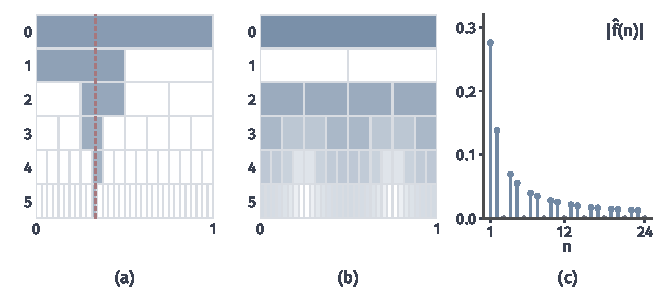
\includegraphics[width=112mm]{figures/04-spaces-measures-and-geometry/03-function-spaces/matplotlib/wavelet-coefficient-tiles/figure.pdf}
  \caption{两种坐标下的系数分布。(a)(b)的每个方格是一个Haar细节系数：纵向为尺度$j$，横向为位置；颜色越深绝对值越大（对数色阶，$10^{-3}$至$1$），白色表示为零。(a)是跳跃函数$\mathbf 1_{[1/3,1)}$，每层只有含跳跃点的一格非零，红色虚线标出$x=1/3$。(b)是$\sin(2\pi x)$，第$1$层全为零，更细的层全部非零。(c)是跳跃函数的Fourier系数绝对值，$n$为$3$的倍数时为零。}
  \label{fig:wavelet-coefficient-tiles}
\end{BookInlineFigure}

\paragraph{平滑振荡}
取$g(x)=\sin(2\pi x)$，$\lVert g\rVert_2^2=1/2$。由$\sin(2\pi x)=(e_1-e_{-1})/(2\mathrm i)$，Fourier系数只有两个非零：
\[
 \hat g(1)=-\frac{\mathrm i}2,\qquad\hat g(-1)=\frac{\mathrm i}2.
\]
两项就精确表示了$g$。

Haar系数则遍布各层。粗项$\int_0^1g=0$。对第$j$层区间$[a,a+h)$，$h=2^{-j}$，记中点$m=a+h/2$，由和差化积，
\begin{equation*}
\begin{aligned}
 \int_a^{m}g-\int_m^{a+h}g
 &=\frac{\cos2\pi a+\cos2\pi(a+h)-2\cos2\pi m}{2\pi}\\
 &=-\frac{2}{\pi}\cos(2\pi m)\sin^2\frac{\pi h}{2}.
\end{aligned}
\end{equation*}
乘以$2^{j/2}$，就得到
\begin{equation}
 d_{j,k}=-\frac{2}{\pi}\,2^{j/2}\cos(2\pi m_{j,k})\sin^2\bigl(\pi2^{-j-1}\bigr).
 \label{eq:wavelet-sine-coefficients}
\end{equation}

逐层读这个公式。$j=0$时$m=1/2$，$d_{0,0}=2/\pi$。$j=1$时两个中点$1/4,3/4$处余弦为零，这一层全为零，因为$g$在每个半周期内关于中点对称。$j\geq2$时中点$(2k+1)2^{-j-1}$都不是$1/4$或$3/4$，这一层的$2^j$个系数全不为零，量级约为$(\pi/2)2^{-3j/2}$，与定理~\ref{thm:wavelet-moment-decay}的Haar估计一致。

\paragraph{局部跳跃}
取$f=\mathbf{1}_{[1/3,1)}$，$\lVert f\rVert_2^2=2/3$。Fourier系数$\hat f(0)=2/3$，$n\neq0$时
\[
 \hat f(n)=\int_{1/3}^1e^{-2\pi\mathrm inx}\,dx=\frac{e^{-2\pi\mathrm in/3}-1}{2\pi\mathrm in}.
\]
取绝对值，得到
\[
 \lvert\hat f(n)\rvert=\frac{\lvert\sin(\pi n/3)\rvert}{\pi\lvert n\rvert}.
\]
$n$是$3$的倍数时为零，其余时为$\sqrt3/(2\pi\lvert n\rvert)$。一处跳跃使无穷多个频率的系数非零，只按$1/\lvert n\rvert$衰减。

Haar系数则高度集中。粗项为$2/3$。若$f$在第$j$层区间上取常值，那里的细节为零，所以每一层只有包含$1/3$的那个区间给出非零系数。沿用第~\ref{sec:wavelet-coefficients-reconstruction}小节的$t_j$：$t_j=1/3$时，$1/3$落在左半，左半减右半的积分是$h/6-h/2=-h/3$；$t_j=2/3$时落在右半，积分是$0-h/3=-h/3$。

于是每层恰有一个非零系数：
\begin{equation}
 d_{j,k}=-2^{j/2}\cdot\frac{h}{3}=-\frac{2^{-j/2}}3.
 \label{eq:wavelet-jump-coefficients}
\end{equation}
能量核对为
\[
 \Bigl(\frac23\Bigr)^2+\sum_{j\geq0}\frac{2^{-j}}9=\frac49+\frac29=\frac23.
\]

\paragraph{有限项的误差}
表~\ref{tab:wavelet-fourier-haar-budget}列出保留部分系数后的平方误差，误差等于被丢弃系数的平方和。Fourier一列保留$\lvert n\rvert\leq N$的项，Haar一列保留粗项与$j<J$的各层，即$P_Jf$。“非零项数”只计实际非零的系数。数值由上面的系数公式求和得到。

\begin{table}[!htb]
\centering
\caption{跳跃函数$f=\mathbf{1}_{[1/3,1)}$与平滑振荡$g=\sin(2\pi x)$在周期区间上的截断平方误差。Fourier保留$\lvert n\rvert\leq N$，Haar保留$V_J$中的全部系数。}
\label{tab:wavelet-fourier-haar-budget}
\begin{tabular}{lccc}
\toprule
表示与截断 & 保留项数 & $f$的非零项数 & $f$的平方误差\\
\midrule
Fourier，$N=4$ & 9 & 7 & 0.0227\\
Fourier，$N=32$ & 65 & 45 & 0.00307\\
Haar，$J=6$ & 64 & 7 & 0.00347\\
\midrule
表示与截断 & 保留项数 & $g$的非零项数 & $g$的平方误差\\
\midrule
Fourier，$N=1$ & 3 & 2 & 0\\
Haar，$J=3$ & 8 & 5 & 0.0252\\
Haar，$J=6$ & 64 & 61 & 0.000401\\
\bottomrule
\end{tabular}
\end{table}

\paragraph{读表}
对跳跃函数，若按固定的项数预算比较，$J=6$的Haar用$64$个位置得到$0.00347$，$N=32$的Fourier用$65$个位置得到$0.00307$，两者相当：线性地截掉高频或细层，误差都大致与项数成反比。

差别出现在“只保留非零系数”时。Haar的$64$个位置中只有$7$个非零，而Fourier要达到同样的误差需要几十个非零项；同样用$7$个非零系数，Haar的误差是$0.00347$，Fourier的误差是$0.0227$。不过，Haar的这一优势要求事先知道跳跃的位置，或者按系数大小自适应地选择保留哪些项。

对平滑振荡，结论反过来：Fourier两项精确表示，Haar在$64$个位置上仍有误差，并且误差每加一层只缩小约四倍，因为Haar只有一个消失矩。换用更光滑、消失矩更多的小波，每层误差下降会更快，但仍不能用有限项精确表示一个正弦。

这说明，正如$\mathbb R^N$中同一个向量在一组基下可能稀疏、在另一组基下可能稠密，函数的稀疏性也不是函数本身的性质，而是函数和基的搭配。哪种表示误差更小，取决于函数（全局振荡还是局部突变）、所用的基以及预算的计法（固定位置还是自适应选取）。这种依赖关系的一般刻画属于第~\ref{chap:function-approximation}章的函数逼近问题。

\section{本章小结}
\label{sec:wavelet-summary}

本章要找一种坐标，让平稳区域的细节接近零，让局部跳变只影响少数系数。小波系数是把函数这条无限维向量换到多尺度标准正交基后读出的坐标，它按尺度$j$和位置$k$排成一张数表。

有限Haar变换给出最简单的回答：对$2^J$个取值反复求平均与半差，得到一个总平均和$2^J-1$个按尺度、位置排列的差值，一处改动在每一层只影响一个系数。把平均与半差乘以$\sqrt2$，变换成为正交矩阵，矩阵的各行就是新的基向量，系数的平方和等于原向量的平方和，逆变换就是转置。

放回区间上，有限变换就是在分段常数函数空间$V_J$中更换标准正交基。到$V_j$的投影是取区间平均；细节空间$W_j=V_{j+1}\cap V_j^{\perp}$由Haar函数张成，记录较粗表示中缺少的左右差异。取值向量要乘以$2^{-J/2}$才是$L^2$坐标，此时保持的是函数的平方积分。

二进阶梯函数在$L^2([0,1])$中稠密，所以粗项加上全部细节构成标准正交基，部分和就是区间平均$P_Jf$，按$L^2$收敛并满足Parseval等式。区间上的粗项不能省略；连续函数的部分和一致收敛，跳跃函数的部分和不一致收敛。

实轴上，正交多分辨率分析把这些结构抽象成嵌套、缩放、平移基、稠密与分离几条要求。尺度函数通过二尺度关系连接相邻层，母小波由二尺度系数写出，证明的关键是把序列按奇偶分成两路，在每个频率上得到$\mathbb C^2$的一组标准正交基。实轴上每层有无限多个位置，粗项在起始层趋于$-\infty$时消失。

消失矩让局部的低次多项式不留痕迹，光滑函数的细节系数因而随层数快速衰减：对$x^2$，Haar的系数是$2^{-3j/2}$的阶，D4的系数精确等于$-(\sqrt3/8)2^{-5j/2}$。小波的光滑性则决定有限项重构是否光滑。

有限区间要处理跨越端点的基函数。周期化给出周期函数空间的标准正交基，零阶矩保留而高阶矩在跨接缝处失效。周期延拓是$L^2$等距同构，却可能在接缝处产生跳跃或折角；反射延拓能消除取值跳跃而不保证导数连续；边界小波在区间内重新构造端点附近的基函数，需要重新核对正交、完备与消失矩。

与Fourier系数比较，全局振荡适合频率坐标，局部跳跃适合尺度位置坐标，哪种误差更小取决于函数、基和预算的计法。截断误差的定量刻画在第~\ref{chap:function-approximation}章研究；第~\ref{chap:besov-spaces}章在本章的周期边界设定下，用小波系数在各层上的大小定义和刻画函数的正则性。

